\section{问题三求解与分析}
\label{sec:q3}
\subsection{问题的描述与分析}
第三问沿用第二问的核心级Task语义及划分、归核和核内顺序三个决策变量，并在各核的读入路径前加入容量为 $1048576$ B 的共享只读 L2。计算依赖与写出要求仍按原图执行，缓存为部分 $\mathrm{COPY\_IN}$ 提供新的服务路径。若读入命中，数据经 L2 带宽池服务；未命中时经DDR服务。每次读入完成时尝试填充，已驻留对象保持原队列位置。由此，哪一次请求能命中取决于全局读入发射、完成与淘汰的交错，并受张量复用关系影响。

图~\ref{fig:q3_overview} 展示本问的分析与求解流程：以第二问完整方案空间为基础，记录真实缓存事件，从观察到的重复未命中或淘汰窗口提出合法核内顺序候选，再用完整执行评价决定是否接受。实验分为三种口径：100 图的第三问主结果，同一第三问方案有无 L2 的配对结果，以及六张定向图在固定方案下的容量、带宽格点。三者分别刻画总体性能、固定方案缓存收益和定向参数响应。
\begin{figure}[htbp]
\centering
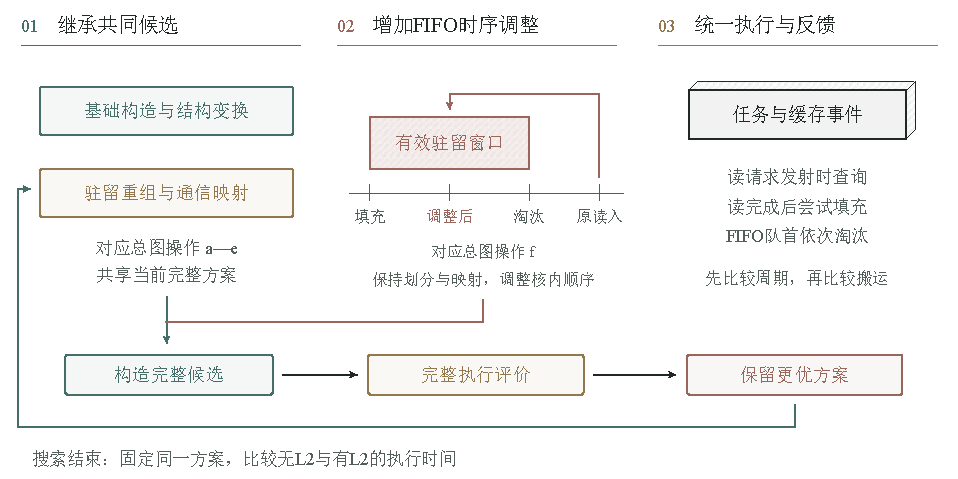
\includegraphics[width=\textwidth]{../求解/问题三/图片/q3_overview.pdf}
\caption{问题三的联合建模与迭代改进框架}\label{fig:q3_overview}
\end{figure}


\subsection{共享只读 L2 的事件模型}
\subsubsection{发射查询、完成填充与 FIFO 顺序}
记全局缓存状态 $\mathcal Q$ 为按成功填入先后排列的逻辑张量标识队列，$B_{\mathrm{L2}}$ 为缓存容量，队列占用按张量字节之和计。同周期事件按执行器次序逐项更新队列。对张量 $t$ 的一次读入请求 $r$，在实际发射时刻 $s_r$ 查询该发射事件之前的队列状态。若命中，则读入由 L2 池服务，并保持 $t$ 的队列位置；若未命中，则请求由 DDR 池服务。每次 $\mathrm{COPY\_IN}$ 在完成时刻 $f_r$ 触发填充尝试：若 $t$ 仍在队列中则保持原状态；若已不在队列且大小可容纳，则依次淘汰队首对象，为 $t$ 腾出空间后插入队尾。尺寸超过容量的张量跳过填充。因此，命中读若在服务期间经历淘汰，也会在完成时重新插入。图~\ref{fig:q3_fifo} 展示查询、路径选择与FIFO填充的处理流程。
\begin{figure}[htbp]\centering
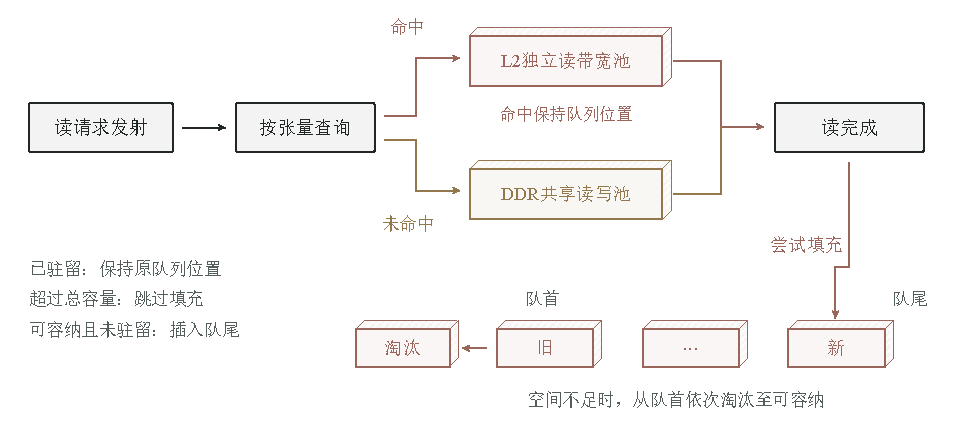
\includegraphics[width=.96\textwidth]{../求解/问题三/图片/q3_fifo.pdf}
\caption{FIFO 读入查询、完成填充与淘汰事件}\label{fig:q3_fifo}
\end{figure}

这一规则尤其影响并发读入。若两核在 $t$ 首次 DDR 读尚未完成时先后发射对 $t$ 的请求，二者查询时 $t\notin\mathcal Q$，因而可以同时未命中。另一方面，已命中的张量即使频繁被读取，也不会因命中刷新 FIFO 位置，后续插入仍可能将其淘汰。已有缓存感知DAG调度研究讨论了节点亲和性与延迟执行对复用的影响\cite{A40}。本题采用FIFO规则，命中由完成填充及后续淘汰形成的驻留区间决定。

第~\ref{subsec:q3_trace_analysis} 节以算例080的张量甲、乙对照这两类时序：甲的后续读取晚于淘汰，乙的一次读取位于驻留期内。缓存时序候选据此尝试调整完整子图的位置，使后续读取有机会落入有效驻留窗口。

\subsubsection{两个共享服务池与计量口径}
设时刻 $\tau$ 在途DDR读写请求集合为 $\mathcal A_D(\tau)$，包括未命中读与写出；在途L2命中读请求集合为 $\mathcal A_L(\tau)$。两池分别以 $60$ B/周期和 $250$ B/周期的总带宽服务，并按各自在途请求数共享；在事件集合不变的区间，某请求以独占服务周期表示的剩余量满足
\begin{equation}
 w_j(\tau+\Delta)=
 \max\!\left\{0,w_j(\tau)-\frac{\Delta}{|\mathcal A_h(\tau)|}\right\},
 \quad j\in\mathcal A_h(\tau),\quad h\in\{D,L\}.
 \label{eq:q3_two_pools}
\end{equation}
两种 $w_j$ 分别按请求所属服务池的带宽换算。DDR 写出和未命中读仍与其他 DDR 请求争用；命中读虽不经 DDR，仍占 L2 池及对应读入流水线，并可能受前驱、缓冲容量和核心内部顺序约束。命中降低该次读的DDR服务需求，其总体收益还取决于请求是否影响关键完成路径。

设 $B_i^{\rm hit}$ 与 $B_i^{\rm miss}$ 为某执行中 \texttt{COPY\_IN} 经 L2 命中和未命中的字节，定义按字节计的命中率
\begin{equation}
 H_i=\frac{B_i^{\rm hit}}{B_i^{\rm hit}+B_i^{\rm miss}}.
 \label{eq:q3_hit}
\end{equation}
当分母非零时，$H_i$ 描述命中字节占全部读入字节的比例。$D_3(x)$ 则按第~\ref{sec:q1} 章的额外COPY口径统计，包括相关的逻辑读入操作。两项指标分别反映服务路径与搬运规模。最终周期还由计算关键链、写出、两池并发以及填充造成的 FIFO 变化共同决定。

\subsection{缓存时序候选与统一接受规则}
\subsubsection{合法顺序邻域}
第三问沿用基础、结构和驻留候选，并增设由已评价缓存轨迹驱动的顺序候选。设当前方案为 $x=(\mathcal P,a,\boldsymbol\pi)$，此来源产生的 $x'=(\mathcal P,a,\boldsymbol\pi')$ 保持算子到子图的划分及子图到核心的归属，只在一个或两个核心的 $\pi_k$ 中移动完整子图。于是原始算子覆盖、每个算子的核心归属与跨核边集合保持不变；但局部先后、读入发射时刻、Spill、FIFO 队列和完成时刻都可能变化。候选随后检查核序与跨核依赖合图的无环性，再作完整执行评价。

从实际未命中记录中，可辨别读入发射时尚有相同张量的在途填充、或上一次缓存副本已被淘汰两类窗口。第一类候选试着将消费者子图后移，或把产生首次有效填充的读者子图前移，让后续发射有机会落在填充之后。第二类候选试着把消费者前移，或把引发实际淘汰的填入者后移，让复用落在淘汰之前。还可联合不同核心上的两次局部移动，并按相邻子图的计算工作量估计需要跨过的时间窗口。移动距离依据原轨迹估计；调整后重新生成所有请求的交错并计算实际命中。候选在来源内去重，经过结构检查、下界筛选和完整执行，才按 $(C_3,D_3)$ 的字典序与当前方案比较。

上述填充与淘汰机制说明，FIFO顺序由成功填入事件决定。静态相邻的消费者仍可能在不同的驻留区间发射请求。来源选择沿用第~\ref{sec:q1} 章的近期收益、运行成本和访问间隔规则，按测量反馈分配有限的搜索机会\cite{A12}。所有来源共享同一当前可行方案，结构或驻留候选被接受后，缓存事件候选会围绕新的执行轨迹重新提出。

\subsubsection{同方案配对的识别量}
令 $x_{i,3,n}$ 为图 $i$、$n$ 核下第三问选出的完整方案。将\emph{同一个方案}分别置于有 L2 和无 L2 的执行环境，定义
\begin{equation}
 R^{\rm L2}_{i,n}=
 \frac{C_2(x_{i,3,n})}{C_3(x_{i,3,n})}.
 \label{eq:q3_pair}
\end{equation}
两次执行保持 $\mathcal P,a,\boldsymbol\pi$ 一致，仅改变缓存规则。式~\eqref{eq:q3_pair} 衡量第三问所选方案的缓存影响；两问各自寻优后的比较则使用各自选出的方案，回答不同的性能问题。

\subsection{主实验与定向参数研究}
\subsubsection{核数扩展、独立优化与同方案对照}
第三问仍用式~\eqref{eq:speedup} 的逐图算术平均。表~\ref{tab:q3_mean} 与图~\ref{fig:q3_mean} 给出一至五核主结果，平均加速比分别为 $1.1008$、$2.1222$、$3.0320$、$3.8376$、$4.5978$，五核中位数为 $4.8565$。一核结果可以高于 1，因为原始单核参考没有按第三问的方案和缓存条件重新优化；多核结果也包含重新分组与顺序的影响。图中的无L2参考曲线也以 $T_{i,0}$ 为分子：对相同第三问方案，逐图计算 $T_{i,0}/C_2(x_{i,3,n})$，再取100图的算术平均。它与有L2曲线使用同一单核基准；固定方案的缓存周期比另由式~\eqref{eq:q3_pair} 给出。
% 由求解/规范化数据/combined/means.csv 生成；逐图加速比的算术平均。
\begin{table}[htbp]
\caption{问题三各核数逐图加速比统计}\label{tab:q3_mean}
\centering\normalsize
\setlength{\tabcolsep}{5pt}
\begin{tabular}{rrrrrr}
\toprule
核心数 & 样本数 & 平均加速比 & 中位加速比 & 最小加速比 & 最大加速比 \\
\midrule
1 & 100 & 1.1008 & 1.0427 & 0.9969 & 2.0540 \\
2 & 100 & 2.1222 & 2.0271 & 1.5225 & 3.6533 \\
3 & 100 & 3.0320 & 3.0182 & 1.7667 & 5.4726 \\
4 & 100 & 3.8376 & 3.9656 & 1.9853 & 7.0949 \\
5 & 100 & 4.5978 & 4.8565 & 2.0717 & 8.7768 \\
\bottomrule
\end{tabular}
\end{table}

\begin{figure}[htbp]\centering
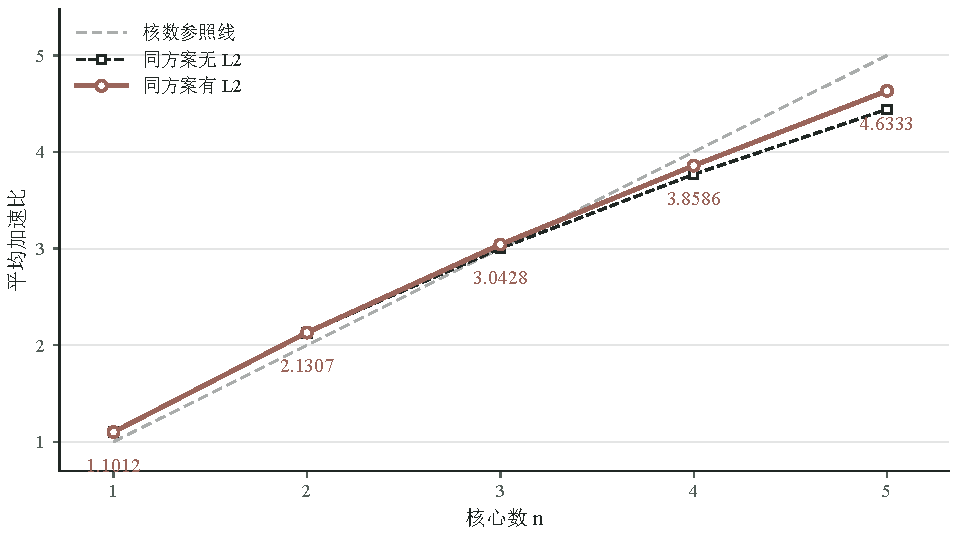
\includegraphics[width=.91\textwidth]{../求解/问题三/图片/q3_mean.pdf}
\caption{第三问各核数主结果及同方案无 L2 参考}\label{fig:q3_mean}
\end{figure}

若改用两问各自选出的五核方案相较，第三问在 100 图中有 66 图周期短于第二问、18 图相等、16 图更长。该对照同时包含两问的执行规则与方案选择差异。第三问五核额外 COPY 字节均值为 $8293721.4$ B，中位数为 $1484117$ B；它们与第二问使用相同的逻辑搬运统计口径。逻辑COPY和自动换出量可能随所选方案变化，读入请求的服务路径则随缓存命中情况变化。

同方案配对覆盖 100 图的全部五种核数，共 500 组。各核数样本量、平均和中位周期比列于表~\ref{tab:q3_pairs}，经验分布见图~\ref{fig:q3_pairs}。五核平均周期比为 $1.0558$，中位数为 $1.0077$；77 图的周期缩短，23 图相等。周期比集中在1附近，说明许多方案的总体完成周期变化较小；右侧尾部对应缓存收益较大的少数算例。
% PR60–62：90组新配对、410组同方案继承；均值是逐例比值的算术平均。
\begin{table}[htbp]
\caption{第三问同一方案有无 L2 的周期配对统计}\label{tab:q3_pairs}
\centering\normalsize
\setlength{\tabcolsep}{4pt}
\begin{tabular}{rrrrrrrr}
\toprule
核数 & 配对数 & \shortstack{平均\\周期比} & \shortstack{中位\\周期比} & 改善 & 相同 & 退化 & \shortstack{平均字节\\命中率} \\
\midrule
1 & 100 & 1.0003 & 1.0000 & 28 & 72 & 0 & 0.0586 \\
2 & 100 & 1.0013 & 1.0001 & 55 & 45 & 0 & 0.1494 \\
3 & 100 & 1.0145 & 1.0004 & 61 & 39 & 0 & 0.2245 \\
4 & 100 & 1.0290 & 1.0019 & 72 & 28 & 0 & 0.2449 \\
5 & 100 & 1.0560 & 1.0082 & 76 & 24 & 0 & 0.3004 \\
\bottomrule
\end{tabular}
\end{table}

\begin{figure}[htbp]\centering
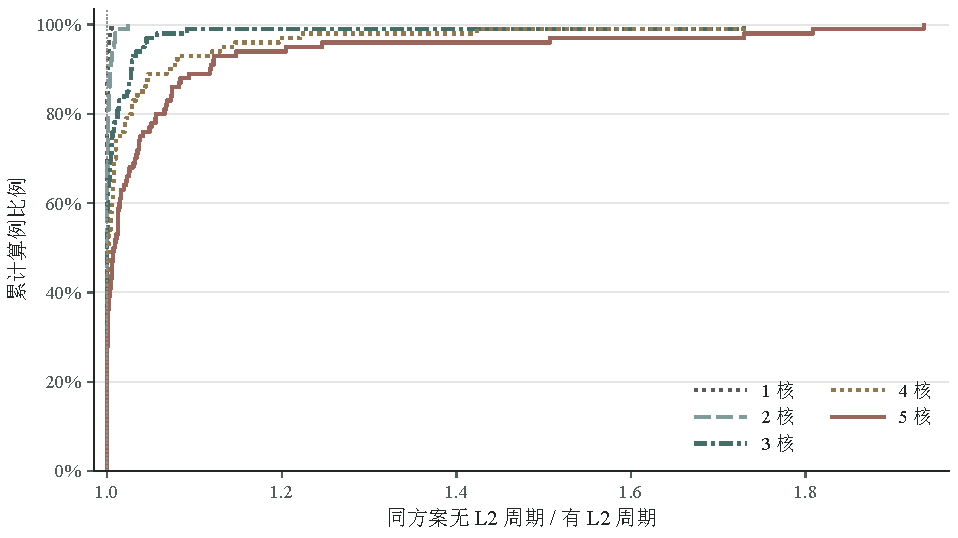
\includegraphics[width=.92\textwidth]{../求解/问题三/图片/q3_pairs.pdf}
\caption{各核数同方案缓存周期比的经验分布}\label{fig:q3_pairs}
\end{figure}

图~\ref{fig:q3_hit_gain} 对照逐例命中字节率与式~\eqref{eq:q3_pair}。解释逐例收益时，需要同时考虑命中位置与事件时序：命中若落在非关键请求上，可能不改变总体任务执行时间；低命中率也可能恰好覆盖关键链上的少量大请求。散点展示了命中率相近的方案仍可能具有不同周期收益的现象。第三问主结果的全局下界与当前五核周期给出的相对差距上界逐图平均为 $0.2248$；其中 6 图在 $1\%$ 以内。该界由计算路径、Pipe负载和对全部可行方案成立的必要流量松弛得到。
\begin{figure}[htbp]\centering
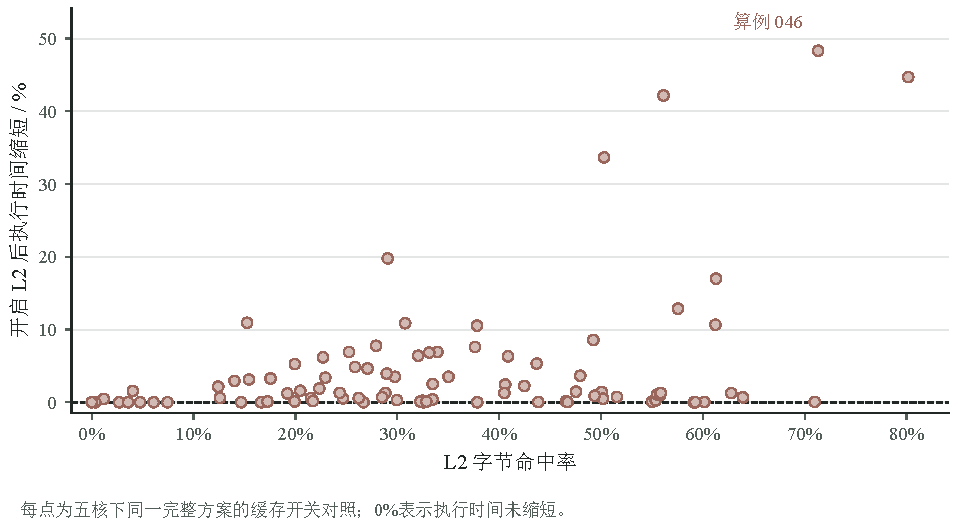
\includegraphics[width=.92\textwidth]{../求解/问题三/图片/q3_hit_gain.pdf}
\caption{字节命中率与同方案缓存周期比}\label{fig:q3_hit_gain}
\end{figure}

\subsubsection{固定方案的容量—带宽响应面}
为观察参数敏感性，从主实验中定向选取六张图，每图固定一份五核完整方案，分别在 L2 容量 $262144$、$1048576$、$4194304$ B，与 L2 带宽 $60$、$250$、$500$ B/周期的九个组合下执行。图~\ref{fig:q3_parameters} 展示共 54 个固定方案格点的真实周期；其中各图的默认配置格沿用对应主实验响应。由于一张图的九格使用同一划分、归核和顺序，格内差异反映该固定方案对参数变化的响应。六个定向算例用于展示不同的缓存机制与敏感性。
\begin{figure}[htbp]\centering
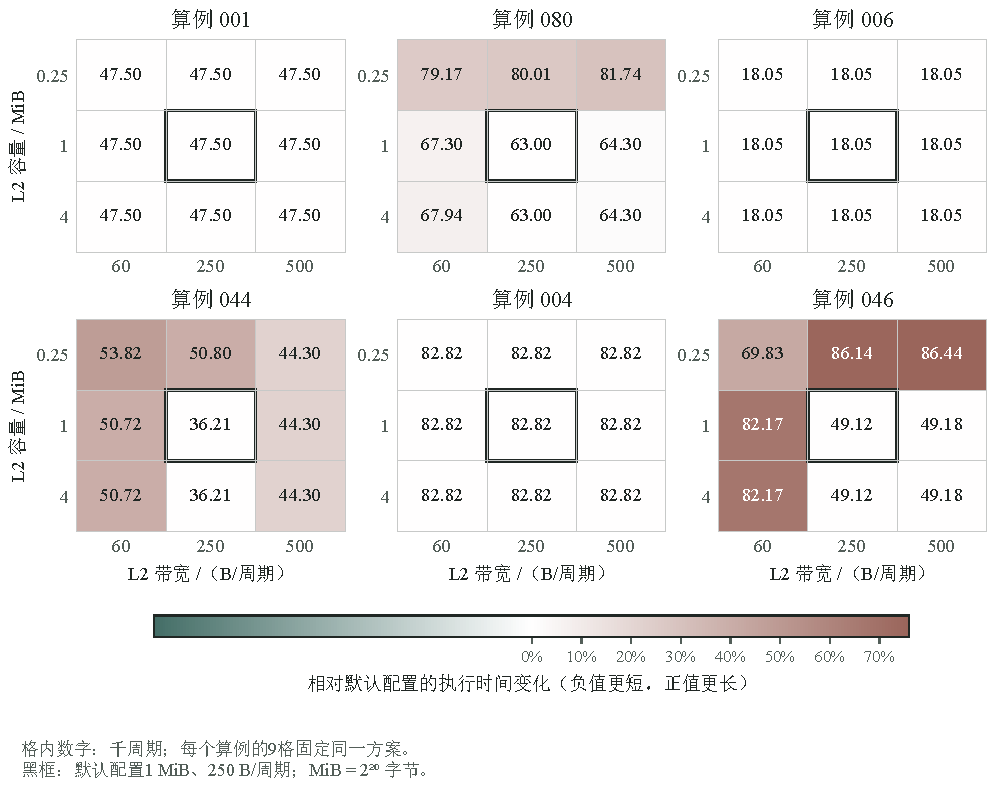
\includegraphics[width=.96\textwidth]{../求解/问题三/图片/q3_parameters.pdf}
\caption{六图固定方案的 L2 容量与带宽周期响应}\label{fig:q3_parameters}
\end{figure}

算例080在带宽固定为 $250$ B/周期时，容量从 $262144$ B 增至 $1048576$ B，周期从 $80014$ 降至 $63001$，字节命中率从 $0.1827$ 升至 $0.5031$。算例001的九个格点均为 $47502$ 周期且零命中，表明提高缓存容量或 L2 带宽只有在相应读入真正利用缓存并影响完成路径时才可能奏效。另在每图的两个边界参数配置下重新适配方案，共取得12个观察值，用于观察参数改变后的重新优化表现；其配置与结果列于支撑材料。

由事件、配对与参数格可见，缓存时序优化需要使关键请求落在有效FIFO驻留窗口内，同时协调L2池与读入Pipe的争用。下面结合具体张量的填充与淘汰事件，分析这些参数响应中的时序差异。

\subsection{缓存驻留窗口的推导与逐事件分析}
\subsubsection{先进先出驻留窗口}
缓存时序候选需要判断一次顺序移动试图跨过哪个事件。考察张量 $t$ 成功填入后、首次淘汰前的一段驻留期，设其大小为 $b_t\le B_{\mathrm{L2}}$。按评估程序的事件次序编号，$e_f$ 表示本次填充事件，$A_t(e)$ 表示从 $e_f$ 之后到事件 $e$ 新插入队尾的对象字节总和。已驻留对象的查询或再次填充不计入，超容量而未入队的对象也不计入。

\textbf{命题4：}若填入只在容量不足时按FIFO顺序淘汰、命中不刷新队列位置，且不发生其他删除，则 $t$ 的首次淘汰事件为：
\begin{equation}
 e_v=\min\{e>e_f:e\text{ 为新填入事件，且 }b_t+A_t(e)>B_{\mathrm{L2}}\}.
 \label{eq:q3_fifo_eviction}
\end{equation}

若集合为空，则本段驻留期内不发生淘汰。

\textbf{证明：}在首次淘汰前，原有对象排在 $t$ 前，新填入对象排在 $t$ 后。设新填入事件 $e$ 之前，$t$ 前方对象的总字节数为 $O_e$，后方为 $A_t(e^-)$，本次插入对象大小为 $b_e\le B_{\mathrm{L2}}$。由于FIFO不会先淘汰 $t$ 后方的对象，有 $A_t(e)=A_t(e^-)+b_e$。此次至少需释放的字节数为：
\[
 R_e=\max\{0,O_e+b_t+A_t(e)-B_{\mathrm{L2}}\}.
\]

前方对象能提供的空间为 $O_e$，故：
\[
 \begin{aligned}
 R_e\le O_e&\ \Longleftrightarrow\ b_t+A_t(e)\le B_{\mathrm{L2}},\\
 R_e>O_e&\ \Longleftrightarrow\ b_t+A_t(e)>B_{\mathrm{L2}}.
 \end{aligned}
\]

第一种情形在移除部分旧前缀后即可填入，$t$ 保留。第二种情形移除全部旧前缀仍不够，队首的 $t$ 随即被淘汰。取第二种情形首次成立的事件即得式~\eqref{eq:q3_fifo_eviction}。

令 $e_r$ 为向使用算子供给该张量的读入请求的发射事件，$\prec$ 表示评估程序中的先后次序。该次读入命中这段驻留期的条件为：
\begin{equation}
 e_f\prec e_r\prec e_v.
 \label{eq:cachewindow}
\end{equation}

若尚未淘汰，把右端点视为无穷远。三个事件的周期分别记为 $f_t,s_t,e_t$。仅在时刻互异时，式~\eqref{eq:cachewindow} 才可简写为 $f_t<s_t<e_t$。同周期的填充、淘汰与查询仍按实际事件次序判断。

式~\eqref{eq:cachewindow} 是固定事件序列的性质。移动子图会改变计算完成、请求发射与带宽共享，进而同时改变 $f_t$、$e_t$ 和 $s_t$。实际方法据原轨迹提出移动方向，再重建整个执行过程。新方案中的驻留窗口随新轨迹重新确定。

\subsubsection{算例080的填充、命中与淘汰}
\label{subsec:q3_trace_analysis}
取参数研究中算例080的五核固定方案，L2 容量为 $262144$ B，带宽为 $60$ B/周期。图~\ref{fig:q3_trace} 上部展示张量甲（4096 B）与张量乙（8192 B）的驻留区间及访问事件，下部放大前1400周期的五核读入轨迹。色带末端箭头表示驻留延续至观察窗以外。
\begin{figure}[htbp]\centering
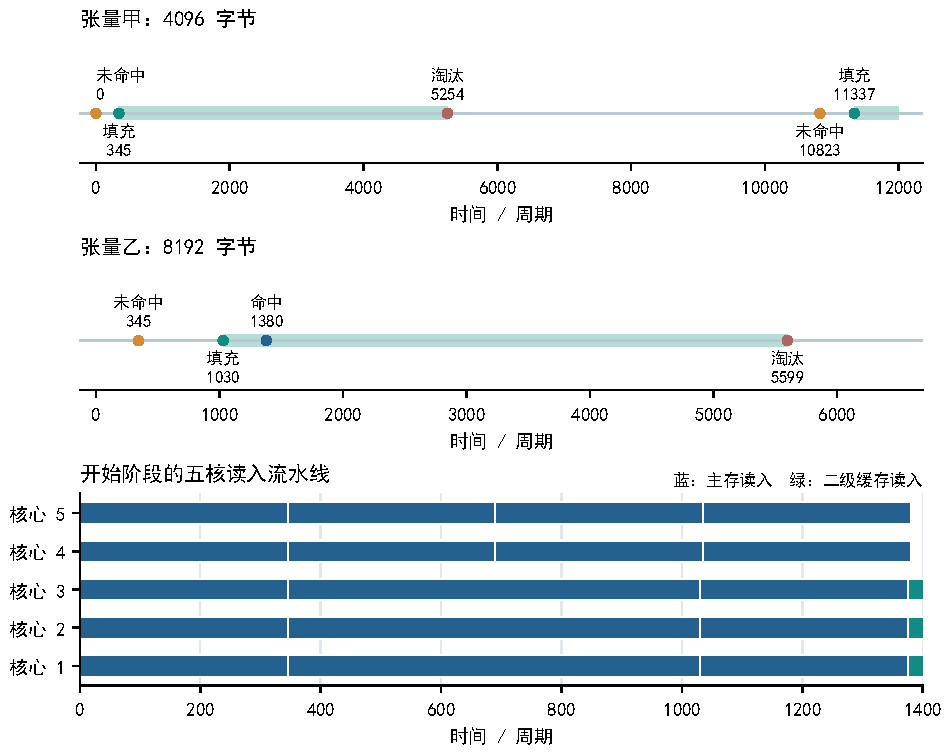
\includegraphics[width=\textwidth]{../求解/问题三/图片/q3_trace.pdf}
\caption{算例080的缓存驻留窗口与多核读入轨迹}\label{fig:q3_trace}
\end{figure}

张量甲在周期0的读取未命中，读入于周期345完成后进入缓存。周期5254的一次新填入将它淘汰。当另一核心在周期10823再次读入甲时，访问已落在这段驻留窗口之外，因此再次未命中。甲在周期11337重新填入，于周期15878再次被淘汰。周期21536的下一次读取仍未命中。

张量乙在周期345查询时未命中，于周期1030填充。周期1380的查询发生在其驻留期内，因而命中。此命中没有将乙移至队尾，周期5599它仍被后续填入淘汰。

图中最早的五个读请求均在周期0发射、周期345完成，显示共享 DDR 上的并发服务。对甲的 $4096$ B 请求，按每请求独占服务周期向上取整得到 $\lceil4096/60\rceil=69$ 周期。在这五个请求同时在途的区间，共享服务使其完成周期与 $5\times69=345$ 一致。

\subsubsection{固定方案的容量与带宽响应}
图~\ref{fig:q3_parameters} 的54个格点保持每张图的五核完整方案不变。算例080在容量 $262144$ B 下，L2 带宽依次为 $60$、$250$、$500$ B/周期时，总体任务执行时间依次为 $79170$、$80014$、$81744$ 周期。对应字节命中率为 $0.1960$、$0.1827$、$0.1680$。带宽提高后，命中率下降而总体任务执行时间上升，表明服务速度的改变伴随缓存访问状态变化。按照前述事件模型，服务完成时刻会影响后续请求发射、缓存填充与淘汰的相对次序。

容量响应也出现平台：算例080在带宽 $250$ B/周期下，容量从 $262144$ B 增至 $1048576$ B 时，周期由 $80014$ 降为 $63001$。继续增至 $4194304$ B，周期仍为 $63001$。算例044在容量 $1048576$ B 下，带宽从 $60$ 增至 $250$、$500$ B/周期，周期为 $50723$、$36208$、$44299$。这两组固定方案结果分别展示了容量增加后的平台和带宽增加后的周期回升，说明需要在完整事件执行中联合评价容量与带宽配置。

算例046五核同方案有L2和无L2的周期分别为 $49119$ 与 $95050$，周期比为 $1.9351$，字节命中率约为 $0.7132$。

